\section{Solvent suppression in NOAH}
\label{sec:noah__solvsupp}

Solvent suppression is one of the most important aspects of modern NMR, and has been incorporated into a large number of experiments.
It is not a particularly difficult task to implement some basic solvent suppression techniques in NOAH supersequences, as will be described in this section.
All suppression techniques shown here can be enabled via acquisition flags (the TopSpin \texttt{ZGOPTNS} parameter); this means that there is no need to switch pulse sequences.


\subsection{Presaturation}
\label{subsec:noah__solvsupp_presat}

A simple first step is to implement simple presaturation of the solvent resonance during the recovery delay of the sequence.
This often provides excellent suppression in the first module in a supersequence, and to a lesser extent, later modules (as the solvent magnetisation recovers during acquisition periods).

Presaturation is also included during long delays, in particular mixing times in NOESY experiments.
The use of presaturation during the HMBC J-evolution delay was also tested, but was found to be generally unnecessary, especially since the HMBC module is typically placed first in supersequences.


\subsection{Intrinsic suppression}
\label{subsec:noah__solvsupp_intrinsic}

A number of NOAH modules in fact come with an \textit{intrinsic} form of solvent suppression, in that they return \magnnot{X} magnetisation (including that of solvents) to the $+z$ axis at the end of the module.
This is generally true of many of the HSQC-based NOAH modules, which seek to only sample \magn{X} magnetisation pool.
Thus, these modules already have far better solvent suppression properties compared to standard library sequences: there is no need for further modification.

For these sequences, it is interesting to go one step further and to see how the solvent suppression varies with transmitter offset.
This is less relevant if the solvent is just water (in which case it suffices to put the water peak on resonance), but may be important for samples in protonated solvents or mixtures thereof.
I tested this by recording the first increment of the NOAH HSQC and seHSQC modules on an aqueous sample of sucrose, and integrating the water peak.
The results (\cref{fig:s_sp_solvsupp}) indicate that the HSQC module provides the best suppression across a range of offsets; of the two seHSQC modules, seHSQC1 provides more uniform suppression, whereas seHSQC2 has some regions (`spikes') where suppression is poorer than average.

\begin{figure}[!ht]
    \centering
    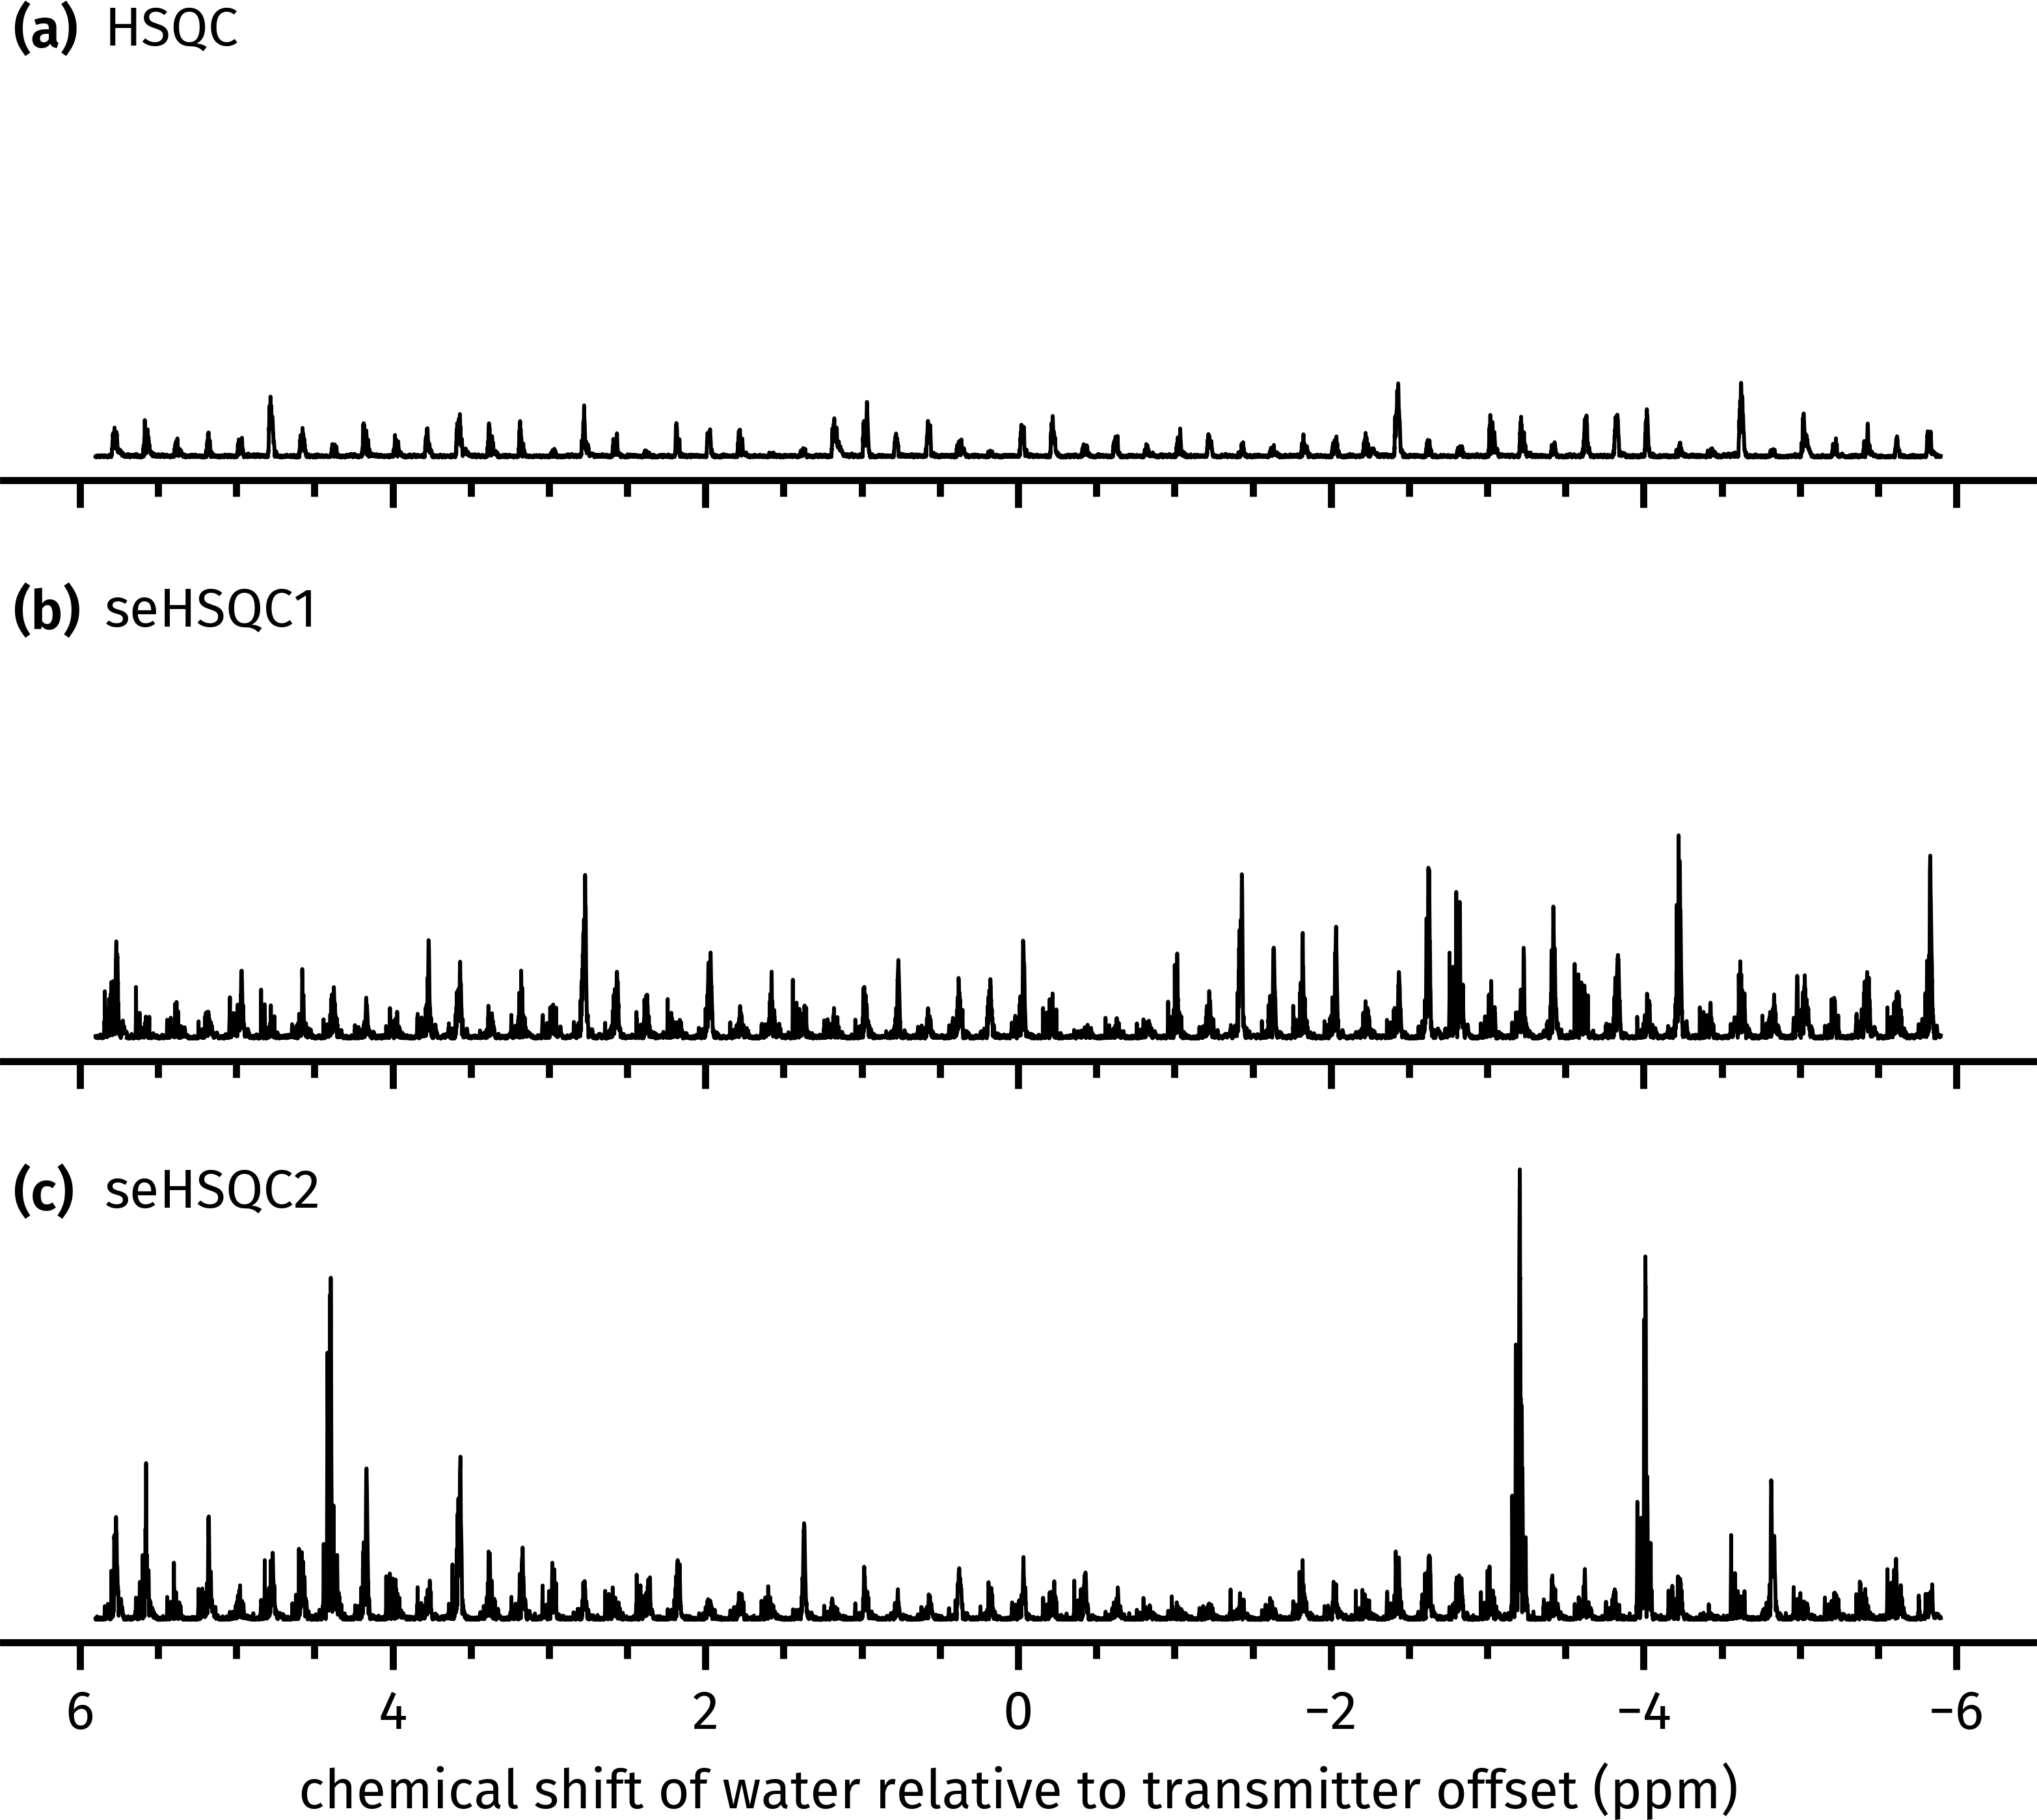
\includegraphics[]{noah/s_sp_solvsupp.png}%
    {\phantomsubcaption\label{fig:s_sp_solvsupp_s}}%
    {\phantomsubcaption\label{fig:s_sp_solvsupp_spv1}}%
    {\phantomsubcaption\label{fig:s_sp_solvsupp_spv2}}%
    \caption[Comparison of solvent suppression in HSQC and seHSQC modules]{
        Residual water peaks observed in the first increment of NOAH HSQC and seHSQC modules, as a function of transmitter offset.
        The $y$-axes of the three subplots are the same.
        \textbf{(\subref*{fig:s_sp_solvsupp_s})} HSQC module.
        \textbf{(\subref*{fig:s_sp_solvsupp_spv1})} seHSQC1 module.
        \textbf{(\subref*{fig:s_sp_solvsupp_spv2})} seHSQC2 module.
        \datacode{7S-201014}
    }
    \label{fig:s_sp_solvsupp}
\end{figure}

It is not surprising that the more complicated seHSQC sequences have slightly poorer suppression: there are substantially more pulses involved which lead to cumulative errors, especially for peaks which are further away from resonance.
However, it is not entirely clear why seHSQC2 has such large spikes.
Some further investigation showed that the poorer suppression partly arises from imperfect cancellation of the water signal by phase cycling.
This is, however, not a full explanation; it merely replaces one mystery with another.
Nevertheless, it should be reiterated that all of these sequences still provide excellent water suppression.
The standard library seHSQC sequences, for example, do not even come close to this level of suppression (although these do dephase water magnetisation prior to acquisition, radiation damping still leads to a very large signal being detected).


\subsection{Excitation sculpting}

Since solvent suppression in HMBC and HSQC-type modules can be adequately accomplished through presaturation and intrinsic suppression, it remains to consider the suppression in homonuclear modules.
These modules invariably occur at the end of supersequences, and thus almost any form of solvent suppression can be used: there is no need to consider how magnetisation needs to be preserved for other modules.

In practice, I chose to implement excitation sculpting\autocite{Hwang1995JMRSA} (ES) just prior to acquisition: the refocusing element chosen was a combination of a selective \ang{180} sinc pulse and a hard \ang{180} pulse.
This worked perfectly for almost all of the homonuclear modules used in NOAH supersequences, with only a few adjustments needed, e.g.\ for the PSYCHE modules to ensure that chemical shifts and J-couplings evolved for the correct amount of time.

The case of the `double' COSY + X homonuclear modules, however, proved to be more intricate.
This is illustrated here using X = TOCSY, but the considerations below are equally applicable to X = NOESY or ROESY.
It is tempting to simply place ES blocks prior to both FIDs: in the COSY module, this dephases transverse solvent magnetisation as desired, and (in principle) should leave longitudinal magnetisation untouched, meaning that the TOCSY module which later consumes this should be unaffected.

However, this is not totally true.
\textit{Inside} the bandwidth of the selective \ang{180} pulse, any longitudinal magnetisation experiences an \ang{720} rotation; and \textit{outside} of the bandwidth, it experiences a \ang{360} rotation.
However, \textit{between} these two extremes, there is a crossover point where longitudinal magnetisation is sent into the transverse plane and subsequently dephased by gradients.
These lead to nulls in \cref{fig:double_es_sim_z}, and peaks which fall within this range will be lost in the TOCSY module.
This is visible in the spectra of \cref{fig:double_es_spec}: although the water suppression obtained using this `double ES' scheme is better, several peaks in the TOCSY spectrum have disappeared, because they fall precisely into these nulls.
It proves better to omit the ES in the COSY module: an adequate degree of water suppression in the COSY can still be attained thanks to the use of presaturation.

\begin{figure}[htb]
    \centering
    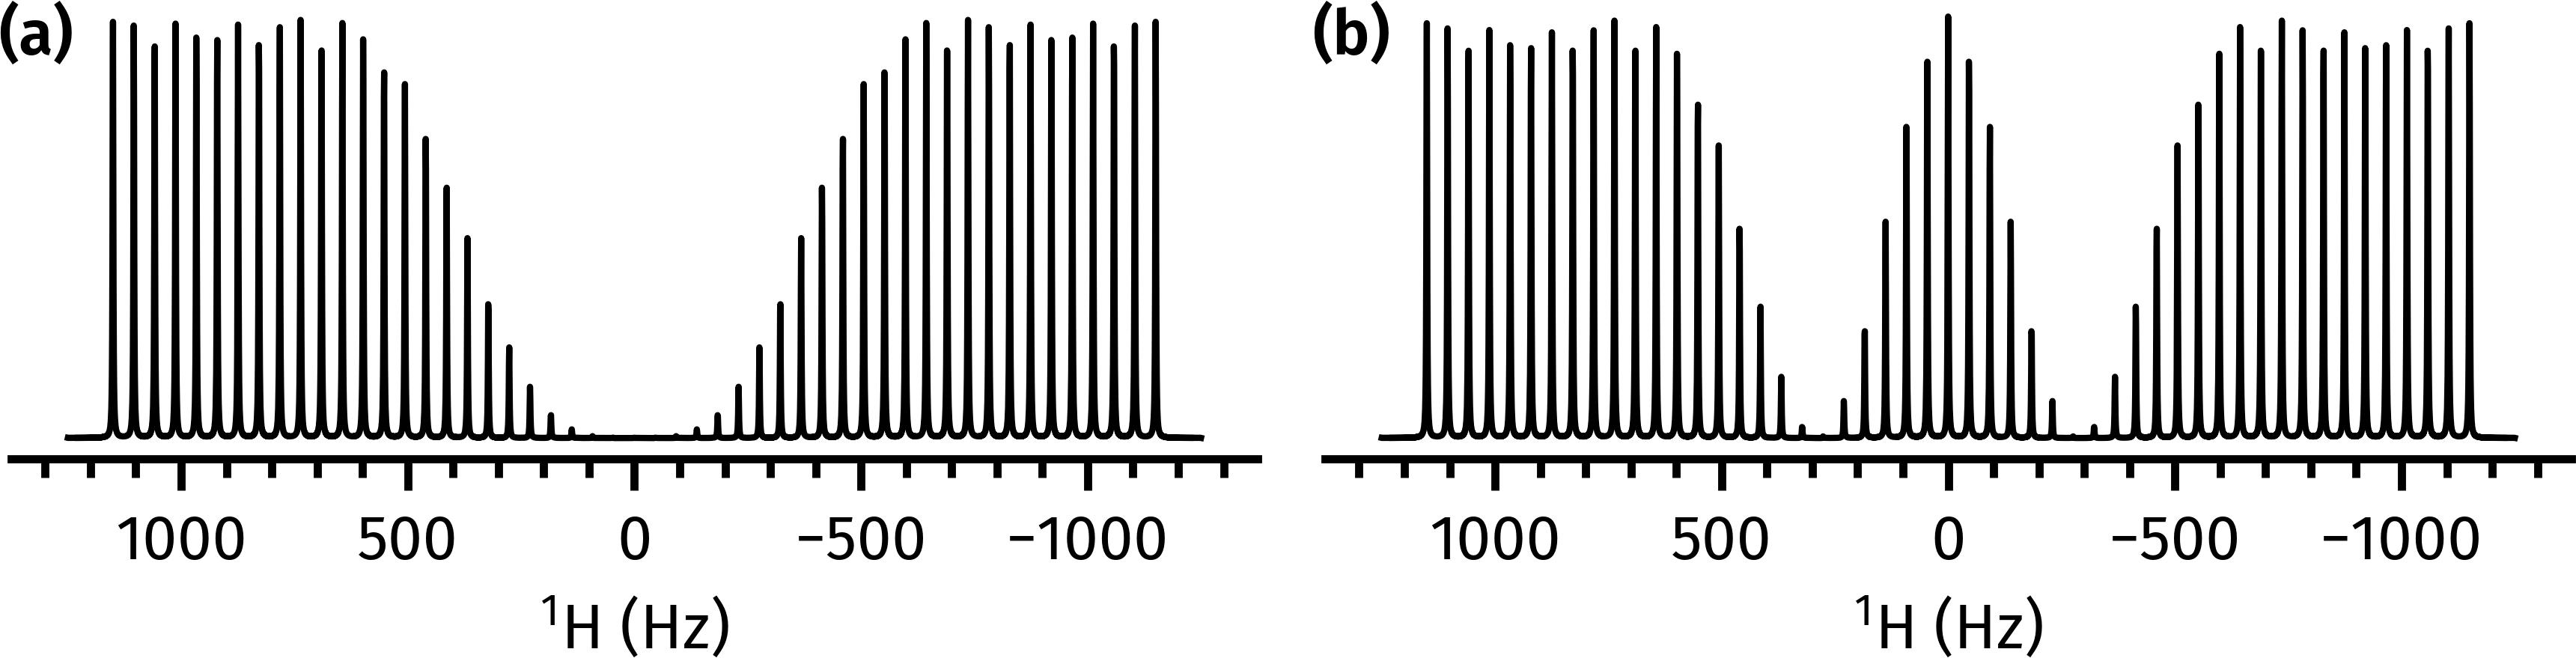
\includegraphics[]{noah/double_es_sim.png}%
    {\phantomsubcaption\label{fig:double_es_sim_xy}}%
    {\phantomsubcaption\label{fig:double_es_sim_z}}%
    \caption[Simulation of magnetisation retained by excitation sculpting block]{
        Simulations showing the proportion of magnetisation retained by the excitation sculpting block (using a \qty{2}{\ms} sinc pulse).
        \textbf{(\subref*{fig:double_es_sim_xy})} Retention of transverse magnetisation: this was obtained by simulating the spectrum of a \ang{90}--ES--detect pulse sequence.
        \textbf{(\subref*{fig:double_es_sim_z})} Retention of longitudinal magnetisation: this was obtained using an ES--\ang{90}--detect pulse sequence.
    }
    \label{fig:double_es_sim}
\end{figure}


\begin{figure}[htb]
    \centering
    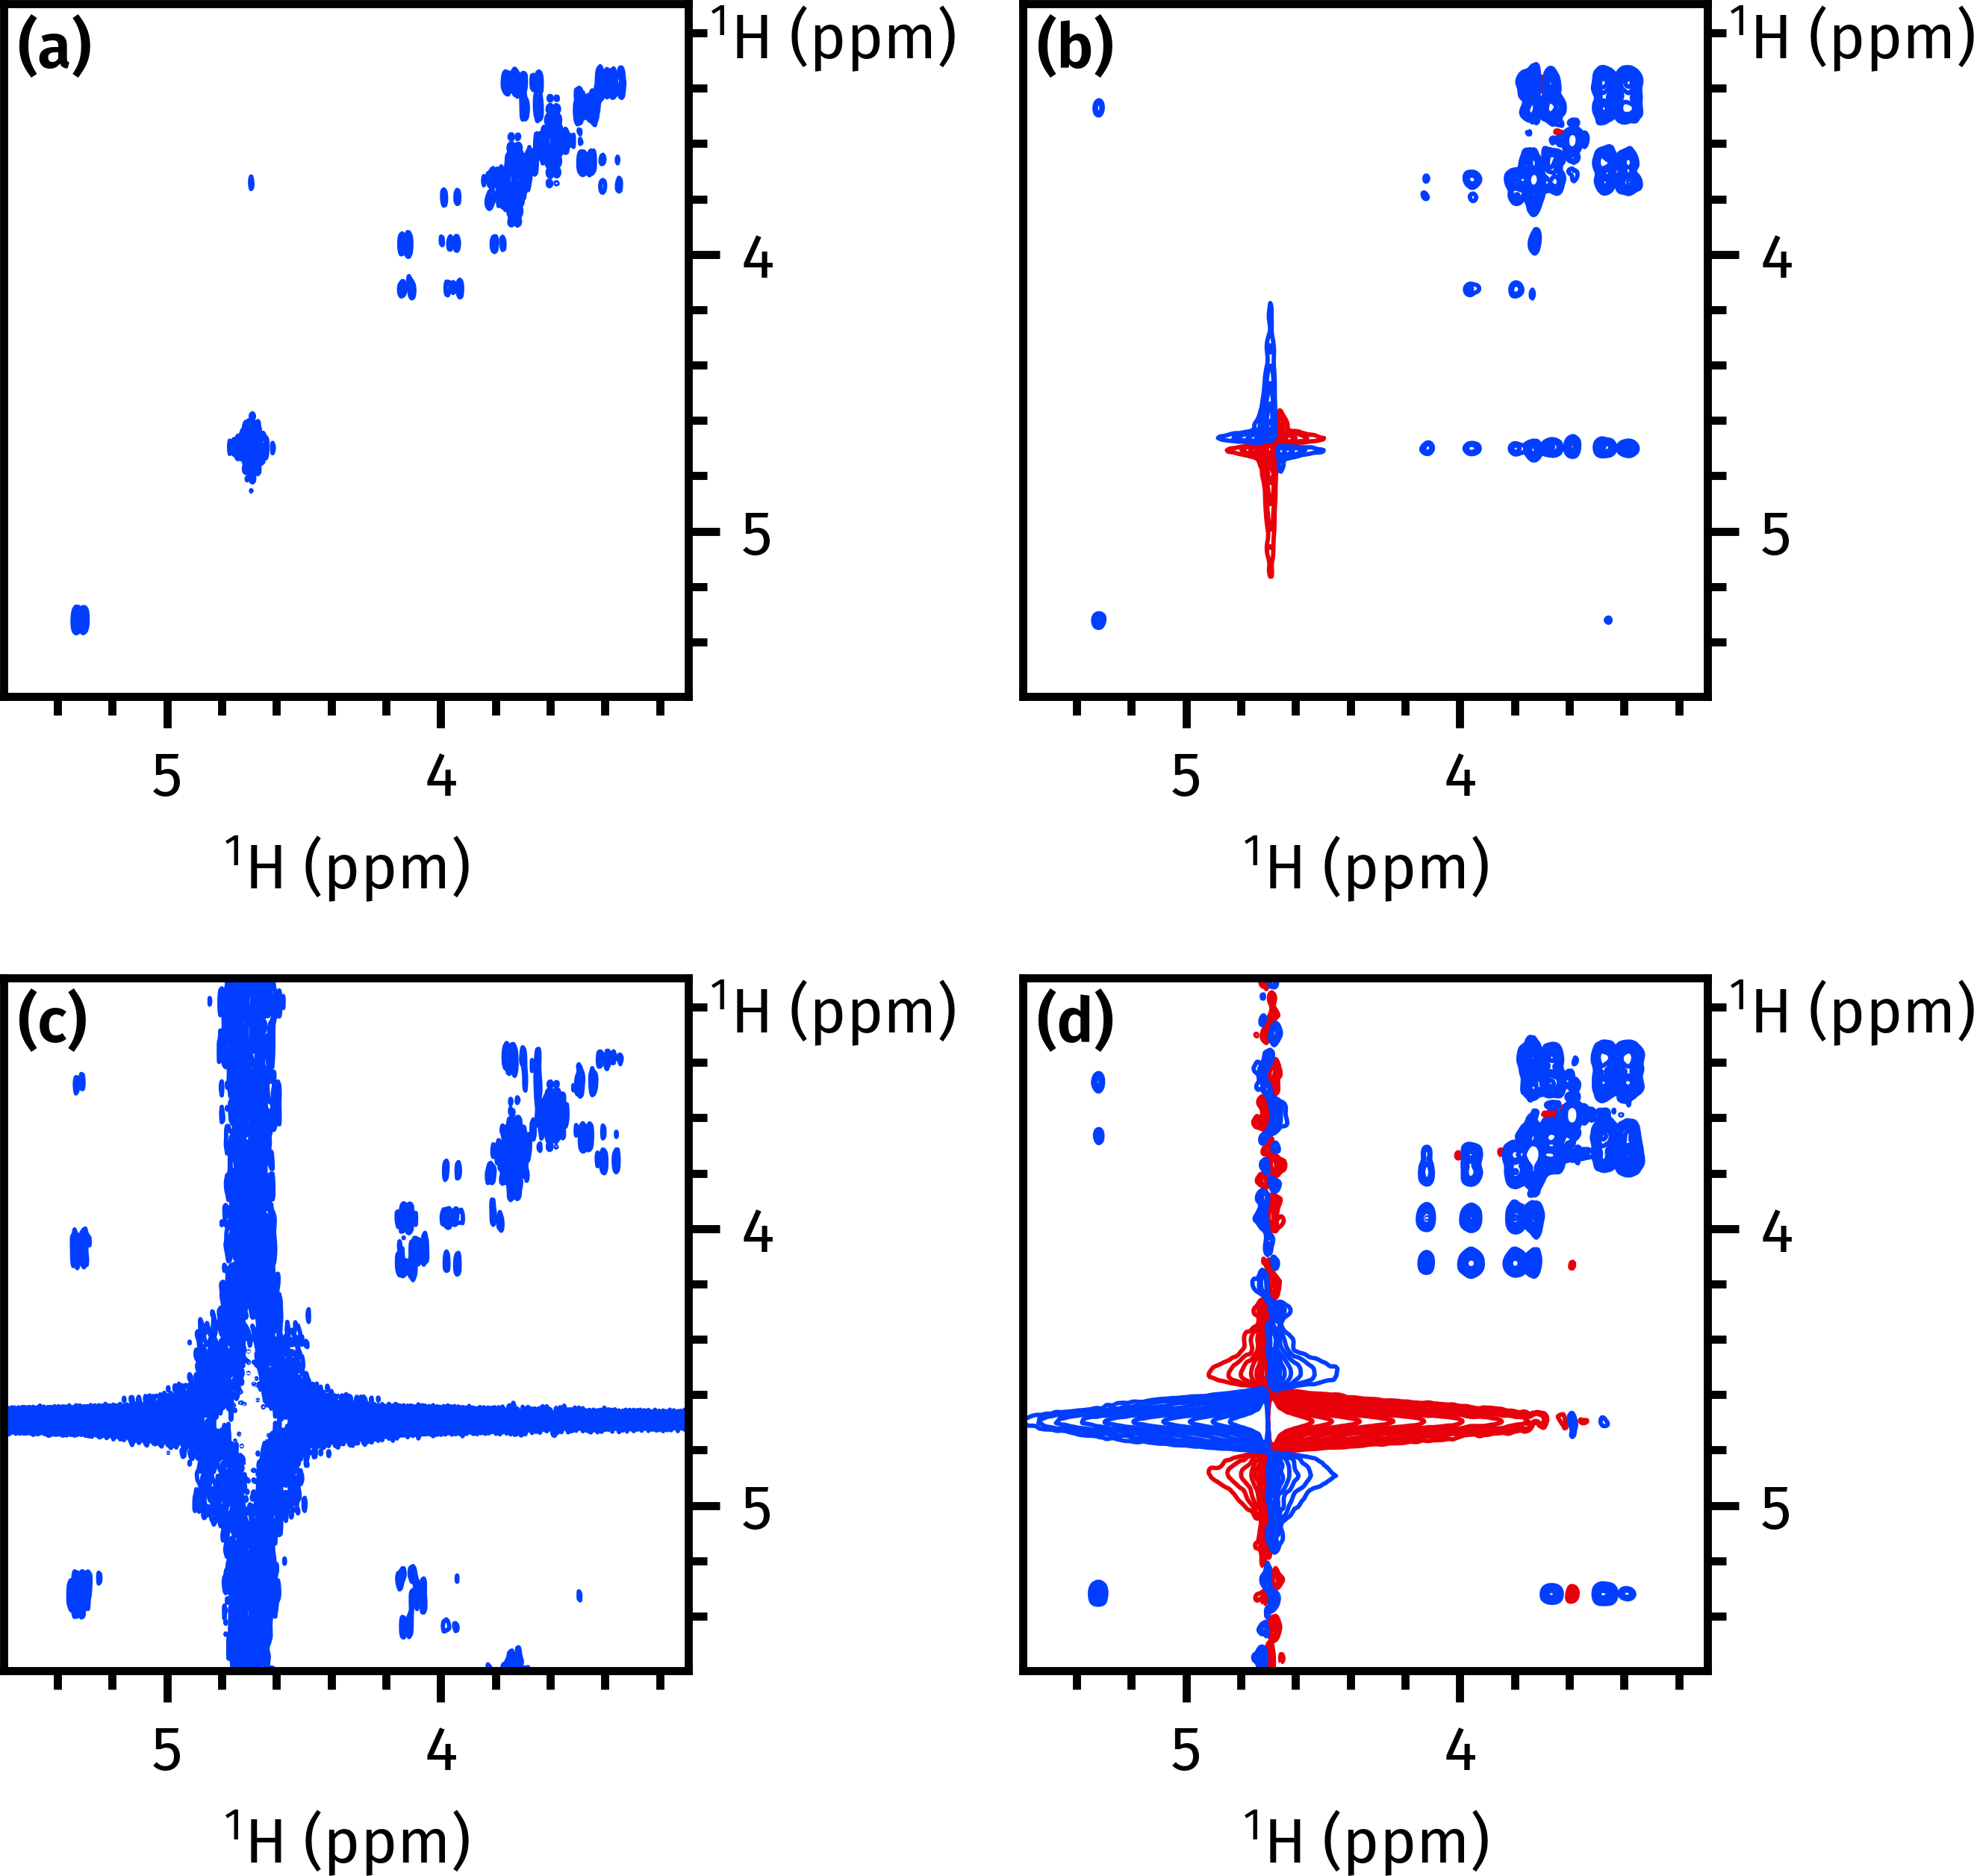
\includegraphics[]{noah/double_es_spec.png}%
    {\phantomsubcaption\label{fig:double_es_spec_2es_c}}%
    {\phantomsubcaption\label{fig:double_es_spec_2es_t}}%
    {\phantomsubcaption\label{fig:double_es_spec_1es_c}}%
    {\phantomsubcaption\label{fig:double_es_spec_1es_t}}%
    \caption[Spectra of CT modules using single and double excitation sculpting]{
        \textbf{(\subref*{fig:double_es_spec_2es_c})--(\subref*{fig:double_es_spec_2es_t})} COSY and TOCSY spectra obtained from a \noah{S,C,T} supersequence where excitation sculpting was placed before both the COSY and TOCSY FIDs.
        Although the water suppression is better, some peaks in the TOCSY module are lost.
        \textbf{(\subref*{fig:double_es_spec_1es_c})--(\subref*{fig:double_es_spec_1es_t})} The same, except that excitation sculpting was applied only in the TOCSY module.
        For all spectra shown here, presaturation of the water resonance was applied during the recovery delay.
        \datacode{4S-211105}
    }
    \label{fig:double_es_spec}
\end{figure}

Of course, it may well be that \textit{no} peaks fall within this null, and thus the better solvent suppression may be obtained at no cost.
This was the case when the experiments in \cref{fig:double_es_spec} were reacquired on a \qty{700}{\MHz} spectrometer; or when the sinc pulse was lengthened to \qty{4}{\ms}.
However, such fortuitousness cannot always be relied on.
